\documentclass[conference]{IEEEtran}
\usepackage{fontspec}
\setmainfont{Times New Roman}
\setmonofont{Courier New}
\usepackage{graphicx}
\usepackage{booktabs}
\usepackage{amsmath}
\usepackage{amsfonts}
\usepackage{amssymb}
\usepackage{url}
\usepackage[hidelinks]{hyperref}
\usepackage{cite}
\usepackage{balance}
\setlength{\textfloatsep}{8pt plus 2pt minus 2pt}
\setlength{\floatsep}{8pt plus 2pt minus 2pt}
\setlength{\intextsep}{8pt plus 2pt minus 2pt}
\renewcommand{\IEEEbibitemsep}{0pt plus .5pt minus 1pt}

\begin{document}

\title{Failure-Aware 2D Aerial Video Mosaicking: An Empirical Study on Indicators, Routing, and Recovery}

\author{
\IEEEauthorblockN{Diep Quang Sang}
\IEEEauthorblockA{\small FPT University\\
Ho Chi Minh City, Vietnam\\
diepqsang13@gmail.com}
\and
\IEEEauthorblockN{Nguyen Duc Nam}
\IEEEauthorblockA{\small FPT University\\
Ho Chi Minh City, Vietnam\\
namnguyen5406gl@gmail.com}
\and
\IEEEauthorblockN{Dao Dang Nguyen Khoi}
\IEEEauthorblockA{\small FPT University\\
Ho Chi Minh City, Vietnam\\
nguyenkhoidao2005@gmail.com}
\and
\IEEEauthorblockN{Truong Quang Dang Khoa}
\IEEEauthorblockA{\small FPT University\\
Ho Chi Minh City, Vietnam\\
Khoa2632006@gmail.com}
}

\maketitle

\begin{abstract}
Sequential 2D aerial video mosaicking from unmanned aerial vehicles (UAVs) relies on incremental homography estimation, which accumulates drift when pairwise registrations degrade over low-texture or repetitive terrain. We present an empirical study of failure-aware mechanisms across eight UAV flight sequences, analyzing 3,898 images (3,890 consecutive pairs) in feature benchmarking and 3,899 images (3,891 steps) in pipeline evaluation. Our findings address three questions without asserting universal pipeline superiority. First, descriptive analysis reveals that point-count heuristics exhibit weak discrimination for step-level registration disagreement (macro Spearman $\rho = -0.091$ and $-0.127$; macro AUC $0.535$ and $0.557$), whereas post-registration metrics---inlier reprojection RMSE ($\rho = 0.728$, AUC $0.882$), zero-mean photometric bad fraction ($\rho = 0.613$, AUC $0.834$), and normalized cross-correlation ($\rho = -0.484$, AUC $0.762$)---correlate more strongly with reference disagreement. Second, an adaptive two-tier matcher router (SIFT with selective escalation to SuperPoint-LightGlue) tuned under Leave-One-Sequence-Out (LOSO) cross-validation with a $\le 25\%$ training escalation budget achieves $2.940$\,px macro step error but requires $813.70$\,s, compared to $261.55$\,s for running SuperPoint-LightGlue everywhere on the evaluated hardware. Third, under a shared trigger, frame dropping and keyframe anchoring retain only $43.42\%$ and $43.75\%$ of frames, while submosaic splitting retains all frames at the cost of partitioning the flight into $795$ submosaics. These results highlight practical trade-offs between retention, continuity, and execution latency.
\end{abstract}

\begin{IEEEkeywords}
UAV video mosaicking, incremental homography, failure prediction, adaptive routing, error propagation, map fragmentation, empirical benchmark.
\end{IEEEkeywords}

\section{Introduction}
\label{sec:intro}

Generating an unreferenced 2D mosaic from low-altitude unmanned aerial vehicle (UAV) video provides rapid situational awareness in disaster response, agricultural monitoring, and environmental inspection~\cite{hwang2026,li2023}. Compared to computationally demanding structure-from-motion (SfM) pipelines, sequential 2D mosaicking concatenates planar projective transformations (homographies) between successive video frames~\cite{map2dfusion}.

However, incremental 2D mosaicking accumulates registration errors sequentially. In an incremental chain, the global coordinate transformation for frame $k$ is formed by compounding inter-frame homographies:
\begin{equation}
H_{0 \leftarrow k} = H_{0 \leftarrow 1} H_{1 \leftarrow 2} \dots H_{k-1 \leftarrow k} = \prod_{j=1}^k H_{j-1 \leftarrow j}.
\label{eq:chain_accum}
\end{equation}
When the camera traverses low-texture landscapes, self-similar vegetation, or near-planar flight segments, pairwise feature matching can degrade. If an inaccurate homography $H_{k-1 \leftarrow k}$ is accepted into the chain, subsequent frames inherit the geometric error, leading to cumulative trajectory drift and visual distortion on the accumulated canvas.

To address these vulnerabilities, practical pipelines incorporate failure awareness across three distinct stages:
\begin{enumerate}
    \item \textbf{Failure Prediction / Detection:} Identifying degraded pairwise registrations before their transformation is committed to the global canvas.
    \item \textbf{Adaptive Resource Routing:} Utilizing lightweight classical matchers by default and selectively escalating to learned models when risk is detected.
    \item \textbf{Failure Recovery:} Selecting an intervention policy (such as dropping corrupted frames, re-anchoring to past keyframes, or splitting into disjoint submosaics) when pairwise matching fails.
\end{enumerate}

Prior literature has investigated heuristics for these components~\cite{hwang2026,li2023,kharismawati2025}, yet their interactions and empirical trade-offs require systematic study. Many existing systems adopt acceptance gates based on raw match counts or RANSAC inlier tallies~\cite{hwang2026}, assuming that higher inlier counts reflect reliable planar transformations. Furthermore, adaptive schemes often assume that classical feature matchers (e.g., SIFT~\cite{lowe2004} or ORB~\cite{rublee2011}) are invariably faster than modern deep matchers (e.g., SuperPoint-LightGlue~\cite{detone2018,lindenberger2023} or LoFTR~\cite{sun2021}), without accounting for hardware-accelerated execution.

In this work, we present an empirical study of failure-aware aerial mosaicking across eight UAV video sequences from the Map2DFusion benchmark~\cite{map2dfusion}. We investigate three core research questions:
\begin{itemize}
    \item \textbf{RQ1 (Failure Prediction):} How do lightweight pairwise indicators correlate descriptively with step-level registration disagreement across diverse aerial scenes, and how do feature-count heuristics compare with post-registration photometric and geometric metrics?
    \item \textbf{RQ2 (Adaptive Matcher Routing):} How does a budget-constrained two-tier matcher router behave across unseen sequences under Leave-One-Sequence-Out (LOSO) cross-validation, and what are its measured runtime costs?
    \item \textbf{RQ3 (Failure Recovery and Fragmentation):} When risk is detected, how do frame dropping, keyframe anchoring, and submosaic splitting trade off frame retention against trajectory continuity and map fragmentation?
\end{itemize}

Feature counts show weaker discrimination than several post-registration indicators in this dataset. Routing has lower macro mean step disagreement than SIFT on each policy's evaluable subset, but its summed computation time is $3.11\times$ that of learned-only matching. Splitting retains all input frames while producing 795 fragments. These observations motivate reporting quality, cost, availability, and connectivity jointly.

\section{Related Work}
\label{sec:related_work}

Incremental 2D aerial mosaicking from unmanned aerial vehicle (UAV) video requires addressing sequential registration, computational resource limits, failure detection, and error mitigation. We organize prior literature into four interrelated domains and establish the scope of our comparative evaluation.

\subsection{Incremental Aerial Mosaicking and Monocular SLAM}
Early and contemporary UAV video mosaicking systems rely predominantly on sequential homography chaining. Hwang et al.~\cite{hwang2026} developed a CPU-based real-time 2D orthomosaic framework using incremental homography estimation with classical feature detectors (SIFT~\cite{lowe2004}, ORB~\cite{rublee2011}) and RANSAC~\cite{fischler1981}, relying on inlier count thresholds to accept inter-frame transformations. Li et al.~\cite{li2023} proposed a real-time incremental video mosaic pipeline for UAV remote sensing incorporating weighted reprojection error optimization, overlap-based keyframe selection, and historical keyframe rematching to mitigate tracking drift. Chen et al.~\cite{chen2022} addressed perspective distortion across varying flight elevations by combining dynamic programming seamline estimation with shape-preserving half-projective warps. To overcome the geometric vulnerability of pure pairwise homography chains, Bu et al.~\cite{map2dfusion} introduced Map2DFusion, coupling direct monocular visual SLAM tracking with keyframe graph optimization and local bundle adjustment. In contrast to full visual SLAM frameworks that maintain 3D map points and solve bundle adjustment, our investigation focuses on lightweight 2D incremental homography pipelines operating under sequential resource limits without global graph optimization.

\subsection{Learned Feature Matching and Efficiency Constraints}
Deep learning has substantially advanced feature matching under challenging illumination and viewpoint changes. DeTone et al.~\cite{detone2018} introduced SuperPoint, a self-supervised framework for joint interest point detection and description. Lindenberger et al.~\cite{lindenberger2023} presented LightGlue, a graph neural network matcher that adaptively prunes unmatchable points and enables early stopping. For detector-free matching, Sun et al.~\cite{sun2021} developed LoFTR using Transformers with coarse-to-fine attention, while Wang et al.~\cite{wang2024} proposed Efficient LoFTR to reduce computational complexity through an aggregated attention mechanism with adaptive token selection and a two-stage correlation layer. For edge deployment, Potje et al.~\cite{xfeat2024} developed XFeat, an architecture tailored for lightweight matching on resource-constrained platforms. Kim and Kim~\cite{kim2025} recently combined classical SIFT extraction with LightGlue to handle large rotational displacements in UAV scenes.

While learned matchers demonstrate high pairwise registration capability, their sequential behavior in continuous UAV video chains exhibits practical trade-offs. In long flight sequences without global bundle adjustment, successive pairwise learned transformations can still accumulate residual subpixel errors across nominal flight segments. This motivates evaluating selective escalation strategies rather than continuous unconstrained invocation.

\subsection{Registration Failure Detection and Uncertainty Estimation}
Zaffar et al.~\cite{zaffar2024} compare retrieval-based uncertainty, learned aleatoric uncertainty, and geometric verification for visual place recognition, and introduce a baseline that uses reference-image poses. Their target is confidence in image retrieval, not accumulated aerial-mosaic drift; this distinction motivates evaluating indicators against an explicitly defined registration-error proxy. Barath et al.~\cite{barath2023} provide reference homographies for benchmarking robust estimators and correspondence filtering methods. Ivashechkin et al.~\cite{ivashechkin2021} introduce VSAC, which uses the concept of independent inliers and adaptive sequential hypothesis verification to improve robust estimation. These works distinguish confidence assessment and robust fitting from the separate problem of managing an accepted transformation over a long chain.

Internal solver outputs are useful acceptance signals~\cite{hwang2026,li2023}, but a small residual on selected correspondences does not by itself establish globally consistent registration. Our study examines whether post-registration appearance consistency and geometric indicators add descriptive evidence beyond point counts; it does not assume that photometric agreement proves geometric correctness.

\subsection{Sequential Error Propagation and Recovery Policies}
When registration degradation occurs, an incremental mapping pipeline requires a recovery strategy to handle the corrupted step. The simplest policy, frame dropping, discards unreliable frames~\cite{hwang2026}. However, discarding frames dilates the temporal baseline between incoming frames and the active mosaic anchor, increasing perspective disparity and potentially triggering subsequent drops. Li et al.~\cite{li2023} addressed this by searching past keyframes for rematching candidates, though successful reconnection depends on spatial trajectory overlap and search window constraints. Kharismawati and Kazic~\cite{kharismawati2025} developed DroneZaic for agricultural UAV videos, using motion clustering to partition long flights into independent submosaics.

Submosaic splitting preserves the entire raw frame inventory by opening new reference frames during severe registration disruptions, though this trades single-canvas metric continuity for localized frame coverage. Conversely, frame dropping preserves continuity within surviving segments but risks discarding substantial portions of the flight when degradation persists. In this work, we compare these recovery policies under unified risk-triggering criteria.


\section{Baseline and Methodology}
\label{sec:methodology}

\subsection{Incremental Homography Baseline}
\label{subsec:baseline_model}

Our baseline 2D mosaicking pipeline adopts a planar homography formulation~\cite{map2dfusion,hwang2026}. Let $I_k$ denote the $k$-th video frame. For each consecutive pair $(I_{k-1}, I_k)$, keypoints and descriptors are extracted and matched. Given a set of correspondence pairs $(p_{k-1}^j, p_k^j)$, the inter-frame homography $H_{k-1 \leftarrow k} \in \mathbb{R}^{3 \times 3}$ is estimated via RANSAC~\cite{fischler1981} with a reprojection threshold of $3.0$\,px:
\begin{equation}
p_{k-1}^j \approx \pi(H_{k-1 \leftarrow k} \tilde{p}_k^j),
\label{eq:homography_proj}
\end{equation}
where $\tilde{p} = [u, v, 1]^T$ represents homogeneous coordinates and $\pi([x, y, z]^T) = [x/z, y/z]^T$ denotes the homogeneous projection.

Transformations mapped to the original image resolution use $D = \operatorname{diag}(W/w,H/h,1)$, where $(w,h)$ and $(W,H)$ are processed and original image dimensions, respectively: $H_{\mathrm{orig}} = D H D^{-1}$. Numerical and geometric acceptance checks in the benchmark do not establish global registration correctness.

Global canvas coordinates are formed by accumulating valid pairwise transformations via Eq.~\eqref{eq:chain_accum}. An affine bounding translation $T$ shifts the origin of $H_{0 \leftarrow k}$ to non-negative coordinates on the global canvas. Overlapping image regions are combined using uniform 50/50 averaging on the canvas.

\begin{figure*}[t]
\centering
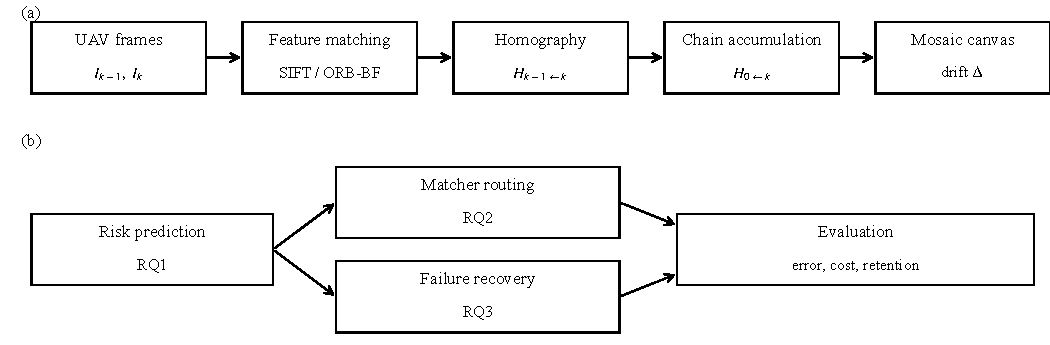
\includegraphics[width=0.96\textwidth]{figures/baseline.pdf}
\caption{System architectural framework. Panel (a) illustrates the standard sequential 2D mosaicking baseline without risk-triggered intervention, where pairwise registration errors accumulate unchecked into the global canvas. Panel (b) illustrates the evaluated modular interventions: step-level risk detection (RQ1), adaptive two-tier matcher routing under LOSO cross-validation (RQ2), and downstream recovery policies (RQ3: none, drop, anchor, split) evaluated under a unified risk trigger.}
\label{fig:baseline_arch}
\end{figure*}

\subsection{Native Baseline and Deep Pilot Observations}
\label{subsec:native_baseline}

To provide an empirical reference, we examine native baseline executions on the 406-frame \texttt{village} sequence at native $1920 \times 1080$ resolution. Table~\ref{tab:native_pilot} summarizes performance across classical SIFT-BF and ORB-BF baselines, alongside deep pilot runs utilizing SIFT-LightGlue and SuperPoint-LightGlue.

\begin{table*}[t]
\centering
\caption{Native Baseline and Deep Pilot Comparison on 406-frame \texttt{village} Sequence (Native Resolution)}
\label{tab:native_pilot}
\footnotesize
\begin{tabular}{lcccc}
\toprule
Configuration & Frames Placed & Total Time (s) & Clock Scope & Canvas Cov. \\
\midrule
SIFT-BF (B) & 406 / 406 & 858.88 & Pipeline total & -- \\
ORB-BF (B) & 406 / 406 & 231.72 & Pipeline total & -- \\
SIFT-LG (P) & 406 / 406 & 1292.46 & Chain total & 82.45\% \\
SP-LG (P) & 406 / 406 & 512.40 & Chain total & 75.15\% \\
\bottomrule
\end{tabular}
\end{table*}

\begin{figure*}[t]
\centering
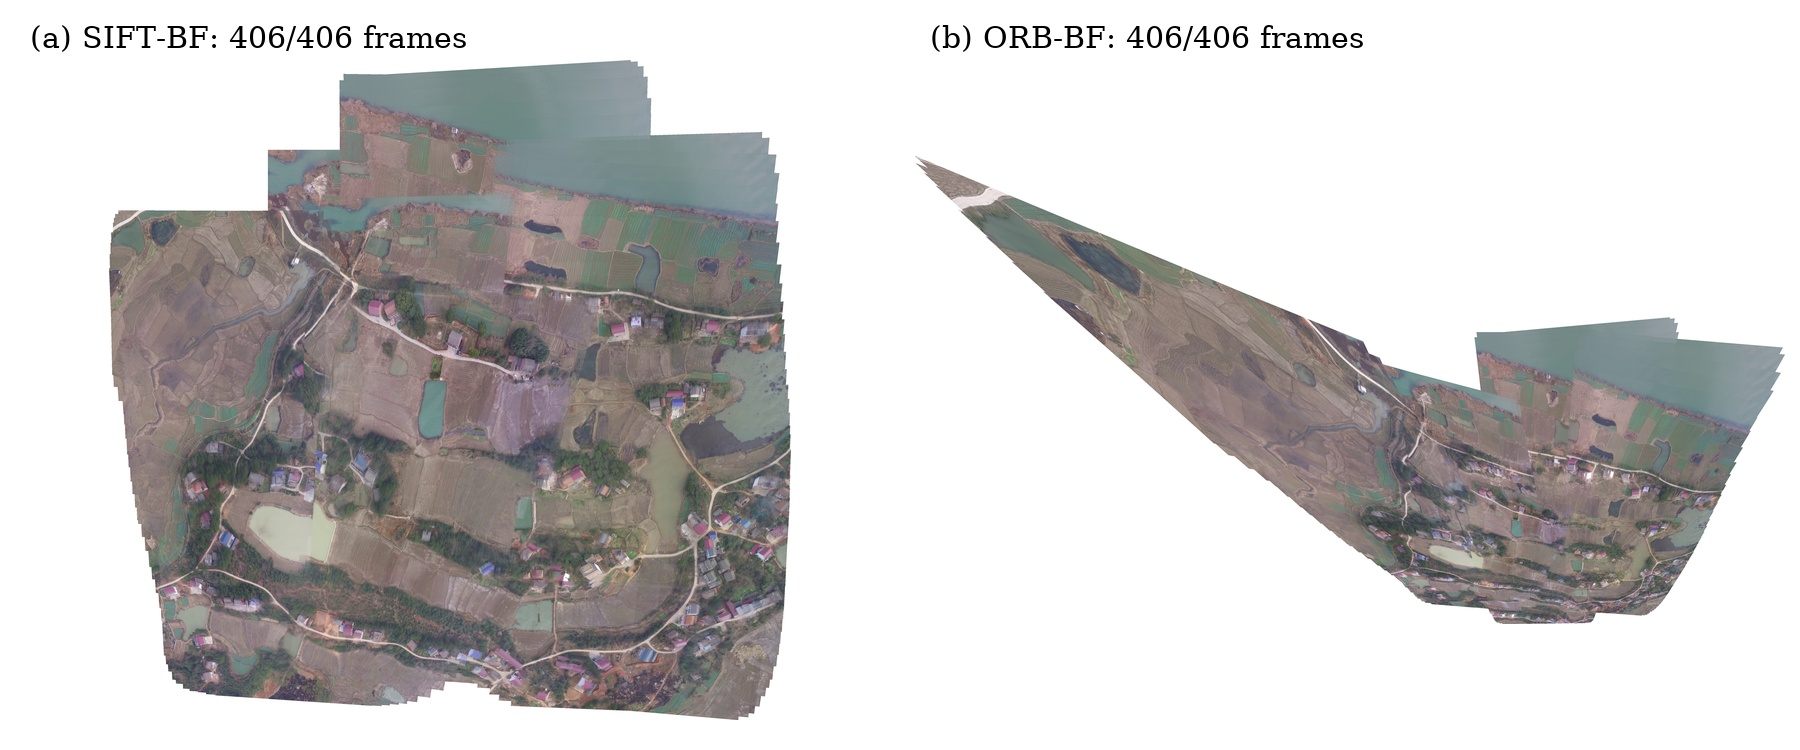
\includegraphics[width=0.88\textwidth]{figures/baseline_mosaics.jpg}
\caption{Qualitative comparison of classical mosaicking baselines on the 406-frame \texttt{village} flight sequence. Panel (a) shows the SIFT-BF reconstruction ($406/406$ frames placed, $858.88$\,s total runtime), which exhibits visible seamline intensity discrepancies and localized shear. Panel (b) shows the ORB-BF reconstruction ($406/406$ frames placed, $231.72$\,s total runtime), which suffers visible elongation and non-linear stretching along flight turns. Both pipelines retain $100\%$ of frames, showing that frame retention alone is an incomplete measure of geometric mapping consistency.}
\label{fig:baseline_mosaics}
\end{figure*}

Both classical baselines place $406/406$ frames, yet their saved canvases exhibit different shapes and visible seams (Fig.~\ref{fig:baseline_mosaics}); retention alone does not establish geometric fidelity. The deep pilot reports canvas coverage of $82.45\%$ (SIFT-LG) and $75.15\%$ (SP-LG). Its chain-total timer is not a matching-only timer and excludes the separate pairwise pilot. These native-resolution records use different execution and timing scopes, so they are not a controlled speedup comparison with the 640\,px benchmark.

\subsection{Pairwise Risk Indicators (RQ1)}
\label{subsec:indicators}

To detect registration degradation at the step level, we evaluate eight indicators:
\begin{enumerate}
    \item \textbf{Point-Count Heuristics:} Raw match count ($N_m$), RANSAC inlier count ($N_{in}$), and inlier ratio $R_{in} = N_{in} / \max(N_m, 1)$.
    \item \textbf{Geometric Distribution:} Inlier convex hull area ratio ($\mathcal{A}_{hull} / (w \cdot h)$) and bounding quad overlap ratio ($\mathcal{O}_{area} / (w \cdot h)$).
    \item \textbf{Post-Registration Consistency:} Inlier reprojection RMSE:
    \begin{equation}
    \text{RMSE} = \sqrt{\frac{1}{N_{in}} \sum_{j=1}^{N_{in}} \| p_{k-1}^j - \pi(H_{k-1 \leftarrow k} \tilde{p}_k^j) \|_2^2},
    \label{eq:rmse_inlier}
    \end{equation}
    and photometric consistency metrics on the backward-warped overlapping domain. Frame $I_{k-1}$ is warped to $I_k$ via $H^{-1}$. On the overlap mask $M$, pixel intensities $x$ (warped) and $y$ (target) are zero-mean centered ($x_p' = x_p - \bar{x}$, $y_p' = y_p - \bar{y}$). Normalized cross-correlation (photo NCC) and photo bad fraction (intensity difference exceeding 25 levels) are computed as:
    \begin{align}
    \text{NCC}(x, y) &= \frac{\sum_{p \in M} x_p' y_p'}{\sqrt{\sum_{p \in M} (x_p')^2 \sum_{p \in M} (y_p')^2} + \epsilon}, \label{eq:ncc} \\
    \text{Frac}_{bad} &= \frac{1}{|M|} \sum_{p \in M} \mathbb{I}(|x_p' - y_p'| > 25). \label{eq:photo_bad}
    \end{align}
\end{enumerate}

\subsection{Adaptive Matcher Routing under LOSO Cross-Validation (RQ2)}
\label{subsec:routing_method}

We evaluate a two-tier routing policy:
\begin{itemize}
    \item \textbf{Tier 1 (Default):} Classical SIFT-BF on 640\,px max-side images.
    \item \textbf{Tier 2 (Escalation):} Deep SuperPoint-LightGlue~\cite{detone2018,lindenberger2023}.
\end{itemize}
The learned-only control uses Tier 2 at every step. Routed-FR keeps the same escalation decisions but uses full-resolution learned matching on escalated steps instead of the 640\,px version.

A step triggers escalation to Tier 2 if any risk condition is met:
\begin{equation}
\begin{aligned}
\text{Trigger}(k)={}&(\text{status}\neq\text{success})\\
 &\lor(\text{NCC}<\tau_{\mathrm{ncc}})\lor(R_{in}<0.30).
\end{aligned}
\label{eq:risk_trigger}
\end{equation}

Under Leave-One-Sequence-Out (LOSO) cross-validation across the eight sequences, sequence $s$ is held out as the test fold. The escalation threshold $\tau_{\mathrm{ncc}}$ is selected from the grid $\{0.90, 0.92, 0.93, 0.94, 0.95, 0.96, 0.97, 0.98, 0.99\}$ on the seven training sequences under the constraint:
\begin{equation}
\tau_{\mathrm{ncc}}^* = \max \left\{ \tau \;\middle|\; \text{Escalation}(s_{train}) \le 25\%, \; \forall s_{train} \right\}.
\label{eq:loso_budget}
\end{equation}
An empty feasible set is recorded as \texttt{infeasible}; diagnostic evaluation then uses the configured fallback $\tau_{\mathrm{ncc}}=0.95$, without claiming budget compliance. All eight reported folds had a feasible training threshold, which was applied unchanged to the held-out sequence. Missing NCC or inlier-ratio values also trigger escalation.

\subsection{Downstream Failure Recovery Policies (RQ3)}
\label{subsec:recovery_method}

When a registration step is flagged as risky by Eq.~\eqref{eq:risk_trigger}, the pipeline invokes a recovery policy. We examine four recovery policies under a fixed matcher baseline:
\begin{enumerate}
    \item \textbf{None (Chaining):} Accepts the candidate homography provided matching succeeded, ignoring the risk trigger.
    \item \textbf{Drop:} Discards frame $I_k$ and attempts to register the next frame to the most recently placed frame, which need not be $I_{k-1}$ after earlier drops.
    \item \textbf{Anchor:} Searches the three most recent previously placed frames excluding the latest placed frame. Their indices need not be consecutive.
    \item \textbf{Split:} Starts a new transform chain with frame $I_k$ as its coordinate origin. Run F records placement and transforms rather than rendering a canvas for each recovery policy.
\end{enumerate}
RQ3 is evaluated on a fixed matcher (SIFT-BF for 7 sequences, EfficientLoFTR for grass), rather than as an end-to-end chained pipeline coupled to RQ2 routing.

\section{Matcher Reference and Experimental Protocol}
\label{sec:protocol}

\subsection{Datasets and Input Accounting}
\label{subsec:datasets}

We evaluate on the Map2DFusion benchmark~\cite{map2dfusion}, containing eight aerial video sequences: \texttt{monticules}, \texttt{npu}, \texttt{saplings}, \texttt{centralPark}, \texttt{factory}, \texttt{grass}, \texttt{huangqi}, and \texttt{village}. Dataset packages include flight trajectory and camera plane metadata, which were intentionally not used in this study to evaluate self-consistency directly from imagery.

\begin{table}[h]
\centering
\caption{Dataset Accounting and Experimental Sequence Profiles}
\label{tab:sequences}
\footnotesize
\begin{tabular}{lrrrr}
\toprule
Sequence & M frames & F frames & Common & Invalid \\
\midrule
monticules & 395 & 395 & 11 & 0 \\
npu & 337 & 337 & 16 & 0 \\
saplings & 482 & 482 & 12 & 0 \\
centralPark & 835 & 836 & 35 & 1 \\
factory & 402 & 402 & 7 & 4 \\
grass & 648 & 648 & 6 & 84 \\
huangqi & 393 & 393 & 27 & 0 \\
village & 406 & 406 & 24 & 0 \\
\bottomrule
\end{tabular}

\end{table}

Images use a maximum side of 640\,px, with dimensions rounded to multiples of 32 (e.g., $1920\times1080$ to $640\times352$). M records a 2,000-keypoint budget for sparse extractors, BF ratio threshold 0.75, RANSAC threshold 3\,px, and EfficientLoFTR confidence threshold 0.2.

Table~\ref{tab:sequences} details the input frame accounting across runs:
\begin{itemize}
    \item Benchmark M contains \textbf{3,898 images} and \textbf{3,890 consecutive pairs}.
    \item Pipeline F contains \textbf{3,899 images} and \textbf{3,891 steps}.
\end{itemize}
The single-image difference arises because pipeline F retained an extra duplicate file in \texttt{centralPark}: \nolinkurl{1454510665.360000 (1).jpg}, which shares an identical SHA-256 hash with the unnumbered file. Benchmark M deduplicated this file, while F processed it. All other 3,898 images match byte-for-byte across runs.

\subsection{Matcher Reference and Gating}
\label{subsec:ref_gating}

In the absence of external geographic ground truth, we utilize a reference matcher: full-resolution SIFT (4,000 keypoints, ratio threshold 0.75, RANSAC threshold 3.0\,px).

To prevent unreliable reference alignments from affecting error measurements, we apply a \textbf{Reference Gate}: a reference homography $H_{ref}$ is accepted only if it achieves $\ge 100$ verified inliers. If $H_{ref}$ has $< 100$ inliers, the step is marked as \texttt{invalid} ($89$ steps in F, including 84 in \texttt{grass}). Step error is evaluated strictly on valid reference steps.

\section{Mathematical Formulation of Metrics}
\label{sec:metrics}

\subsection{Step-Level Registration Disagreement}
\label{subsec:metric_step_error}

Let $H_{est}$ denote the estimated pairwise homography scaled to original resolution, and let $H_{ref}$ denote the valid reference homography. We evaluate geometric divergence across five pixel anchor points $\mathcal{S} = \{ (0, 0), (W, 0), (W, H), (0, H), (W/2, H/2) \}$ representing the image corners and center:
\begin{equation}
E_{step}(H_{est}, H_{ref}) = \frac{1}{5} \sum_{p \in \mathcal{S}} \| \pi(H_{est} \tilde{p}) - \pi(H_{ref} \tilde{p}) \|_2.
\label{eq:step_error}
\end{equation}
A step is labeled as a disagreement step if $E_{step} > 2.0$\,px. Across 3,794 valid evaluation steps, 1,075 steps ($28.33\%$) exceed this threshold for classical SIFT.
RQ1 reports per-sequence Spearman correlation and ROC-AUC, then macro averages. Risk-score directions are fixed by indicator semantics (larger RMSE/photo bad fraction, smaller counts/ratios/NCC); AUC is not flipped post hoc to exceed 0.5. AUC is undefined for single-class sequences.

\subsection{Chain-vs-Direct Common-Frame ATE}
\label{subsec:metric_ate}

To evaluate accumulated drift, we employ a \textbf{Chain-vs-Direct Consistency Metric}. For frame $k$, the accumulated chained homography $H_{0 \leftarrow k}^{chain}$ is compared against a direct registration $H_{0 \leftarrow k}^{direct}$ to frame 0 using full-resolution SIFT.

We define the \textbf{Common Eligible Frame Set} $\mathcal{C}$ as the subset of frames where:
\begin{enumerate}
    \item Direct registration $H_{0 \leftarrow k}^{direct}$ achieves $\ge 100$ inliers.
    \item All seven evaluated matchers maintain an unbroken chain to frame $k$.
\end{enumerate}
The common set excludes frame 0 and is formed separately for each sequence; there are 138 eligible frames in total. Define $e_k=E_{step}(H_{0\leftarrow k}^{chain},H_{0\leftarrow k}^{direct})$. The artifact's common ATE is the pixel-domain root mean square:
\begin{equation}
\text{ATE}_{common}=\sqrt{|\mathcal{C}|^{-1}\sum_{k\in\mathcal{C}}e_k^2}.
\label{eq:common_ate}
\end{equation}
Despite its name, this is image-transform disagreement, not ground-truth trajectory error in metres.

\subsection{Reference-Chain Drift and Recovery Accounting}
Run F instead compares estimated transforms with an accumulated chain of valid reference transforms, using the same five-point distance. This is not the chain-vs-direct metric of run D. An invalid reference edge makes later global-chain comparisons unavailable; opening a submosaic establishes a new local reference origin. The last available value is reported with its frame index, and roots are excluded from drift summaries.

Retention divides placed frames, including roots, by requested input frames. Linked frames have a placement edge; thus retained frames equal linked frames plus submosaic roots. Fragment counts, largest-fragment size, singleton counts, and available non-root drift measurements are reported alongside retention. The \texttt{frames\_requested} field in D describes already-stitched input, so dataset retention uses the original 3,898-frame denominator from M, not D.

\subsection{Macro vs. Pooled Aggregation}
\label{subsec:metric_aggregation}

To prevent longer sequences from dominating aggregate values, we report macro metrics across sequences:
\begin{equation}
\text{Macro}(X) = \frac{1}{N} \sum_{s=1}^N X_s,
\label{eq:macro_mean}
\end{equation}
Pooled metrics instead aggregate observations across sequences. Macro step error is the unweighted mean of sequence-level means over evaluable successful steps. SIFT's 11 missing homographies are excluded from its error calculation; SIFT and routing therefore use their respective evaluable subsets, not an identical sample.

\subsection{Latency Accounting}
\label{subsec:metric_latency}

Timing measurements use monotonic timers with CUDA synchronization (\texttt{torch.cuda.synchronize()}) to avoid asynchronous queuing bias:
\begin{equation}
t_{step} = t_{match} + t_{geo},
\label{eq:time_accounting}
\end{equation}
where $t_{match}$ covers feature extraction and matching, and $t_{geo}$ covers RANSAC fitting, indicator computation, and coordinate scaling. File I/O is excluded from algorithmic latency comparisons.
Routing time sums the default computation at every step and the learned computation at escalated steps. These costs are replayed from saved measurements, not measured end-to-end pipeline wall-clock times.

\section{Empirical Results and Analysis}
\label{sec:results}

\subsection{Overall 7-Matcher Benchmark}
\label{subsec:benchmark_results}

Table~\ref{tab:benchmark} presents the benchmark across seven feature matchers on 3,898 images and 3,890 consecutive pairs.

\begin{table*}[t]
\centering
\caption{Overall Feature Matcher Benchmark Across Eight UAV Video Sequences}
\label{tab:benchmark}
\footnotesize
\begin{tabular}{lrrrrr}
\toprule
Matcher & Pairs & Match (s) & RMSE & Frames & C-ATE \\
\midrule
SIFT-BF & 3875 & 0.220 & 0.559 & 3740 & 49.15 \\
ORB-BF & 3889 & 0.054 & 1.096 & 3535 & 170.51 \\
SIFT-LG & 3889 & 0.329 & 0.628 & 3766 & 45.08 \\
SP-LG & 3889 & 0.067 & 1.282 & 3694 & 83.13 \\
XFeat-MNN & 3888 & 0.019 & 1.353 & 3071 & 138.29 \\
XFeat-LG & 3888 & 0.044 & 1.311 & 3391 & 59.12 \\
ELoFTR & 3884 & 0.184 & 0.917 & 1062 & 3143.64 \\
\bottomrule
\end{tabular}

\end{table*}

Key observations from Table~\ref{tab:benchmark}:
\begin{itemize}
    \item \textbf{Pairwise Success vs. Mosaic Stability:} All matchers achieve $\ge 3{,}875 / 3{,}890$ pairwise matching success. However, downstream mosaic completion varies. EfficientLoFTR (ELoFTR) achieves 3,884 successful pairwise matches with $0.917$\,px inlier RMSE, but completes 0/8 full sequences, placing 1,062 total frames with a macro Common ATE of $3{,}143.64$\,px. This indicates that inlier residuals on isolated pairs do not necessarily reflect multi-frame trajectory stability.
    \item \textbf{SIFT-LightGlue Consistency:} SIFT-LightGlue achieves the lowest macro Common ATE ($45.08$\,px) and retains $3{,}766 / 3{,}898$ frames, completing 7/8 sequences, with a matching latency of $0.329$\,s/pair.
    \item \textbf{XFeat Speed-Stability Trade-off:} XFeat-MNN is the fastest matcher ($0.019$\,s/pair), with lower frame retention ($3{,}071$ frames, 5/8 sequences completed) and higher drift ($138.29$\,px). XFeat-LighterGlue reduces drift to $59.12$\,px at $0.044$\,s/pair, completing 4/8 sequences.
\end{itemize}

\subsection{RQ1: Failure Prediction and Risk Indicators}
\label{subsec:rq1_results}

Table~\ref{tab:rq1} summarizes the predictive capability of the eight evaluated indicators for identifying step disagreement ($E_{step} > 2.0$\,px) on SIFT-BF across 3,794 valid steps.

\begin{table}[h]
\centering
\caption{Step-Level Failure Prediction Metrics for SIFT-BF (3,794 Valid Evaluation Steps Across Eight Sequences)}
\label{tab:rq1}
\footnotesize
\begin{tabular}{lrr}
\toprule
Indicator & $\rho$ & AUC \\
\midrule
RMSE & 0.728 & 0.882 \\
Photo bad fraction & 0.613 & 0.834 \\
NCC & -0.484 & 0.762 \\
Hull area ratio & -0.449 & 0.731 \\
Overlap ratio & -0.452 & 0.720 \\
Inlier ratio & -0.356 & 0.716 \\
Inlier count & -0.127 & 0.557 \\
Match count & -0.091 & 0.535 \\
\bottomrule
\end{tabular}

\end{table}

Key observations from Table~\ref{tab:rq1}:
\begin{itemize}
    \item \textbf{Weak Discrimination of Point Counts:} Inlier count and raw match count exhibit weak Spearman correlation with step disagreement ($\rho = -0.127$ and $-0.091$) and near-random classification performance (macro AUC $0.557$ and $0.535$).
    \item \textbf{Post-Registration Metrics:} Inlier reprojection RMSE exhibits the highest correlation ($\rho = 0.728$, AUC $0.882$), followed by zero-mean photo bad fraction ($\rho = 0.613$, AUC $0.834$) and photo NCC ($\rho = -0.484$, AUC $0.762$). Hull area ratio ($\rho = -0.449$, AUC $0.731$) and overlap ratio ($\rho = -0.452$, AUC $0.720$) provide secondary signals.
    \item \textbf{Scene-Dependent Indicator Variance:} Sequence-level AUCs for photo NCC vary across scenes: $0.636$ (\texttt{monticules}), $0.672$ (\texttt{saplings}), $0.721$ (\texttt{grass}), $0.754$ (\texttt{factory}), $0.803$ (\texttt{npu}), $0.803$ (\texttt{huangqi}), $0.838$ (\texttt{village}), and $0.871$ (\texttt{centralPark}).
    \item \textbf{Degenerate One-Class Case (EfficientLoFTR):} For EfficientLoFTR, $3{,}796$ out of $3{,}802$ valid steps exceeded $2.0$\,px. In seven sequences, zero steps were classified as good, rendering ROC-AUC undefined. On \texttt{centralPark}, only six steps were classified as good, producing an apparent single-sequence AUC of $0.996$.
\end{itemize}

\subsection{RQ2: Adaptive Routing under LOSO Cross-Validation}
\label{subsec:rq2_results}

Table~\ref{tab:routing} reports the performance of our adaptive two-tier routing policy under Leave-One-Sequence-Out cross-validation across 3,891 steps.

\begin{table}[h]
\centering
\caption{Adaptive Matcher Routing Performance Under LOSO Cross-Validation (3,891 Steps)}
\label{tab:routing}
\footnotesize
\begin{tabular}{lrrrr}
\toprule
Policy & Failed & Esc. & Time (s) & Error (px) \\
\midrule
SIFT & 11 & 0 & 792.03 & 6.676 \\
SP-LG & 0 & -- & 261.55 & 3.338 \\
Routed & 0 & 315 & 813.70 & 2.940 \\
Routed-FR & 0 & 315 & 974.95 & 2.843 \\
\bottomrule
\end{tabular}

\end{table}

The LOSO protocol selected $\tau_{\mathrm{ncc}}^* = 0.92$ when \texttt{saplings} was held out, and $\tau_{\mathrm{ncc}}^* = 0.90$ across the other seven folds. The router triggered escalation on $315$ steps ($8.10\%$) across the dataset.

\begin{table}[t]
\centering
\caption{Per-Sequence Routing: Escalated Steps, Trajectory Drift (px), and Last Evaluable Step}
\label{tab:routing_breakdown}
\footnotesize
\begin{tabular}{@{}lcccc@{}}
\toprule
Sequence & Escalated & Classical & Routed & Last \\
\midrule
monticules & 2 / 394 & 3904.57 & 2490.70 & 394 / 394 \\
npu & 26 / 336 & 458.72 & 458.88 & 336 / 336 \\
saplings & 126 / 481 & 5992.82 & 8066.21 & 481 / 481 \\
centralPark & 32 / 835 & 270.43 & 107.40 & 834 / 835 \\
factory & 58 / 401 & 2227.57 & 1630.50 & 375 / 401 \\
grass & 49 / 647 & 3.46 & 3.46 & 18 / 647 \\
huangqi & 2 / 392 & 65.25 & 87.13 & 392 / 392 \\
village & 20 / 405 & 565.68 & 494.11 & 405 / 405 \\
\bottomrule
\end{tabular}
\end{table}

Observations from Table~\ref{tab:routing} and Table~\ref{tab:routing_breakdown}:
\begin{enumerate}\setlength{\itemsep}{1.5pt}\setlength{\parskip}{0pt}
    \item \textbf{Measured Computation Costs:} SIFT costs $792.03$\,s, learned-only SuperPoint-LightGlue $261.55$\,s, and routing $813.70$\,s in summed measurements. Thus routing costs $3.11\times$ learned-only; the intended default matcher is not the cheaper option in this run. No hardware ablation isolates the cause of this ordering.
    \item \textbf{Generalization and Adverse Drift:} On unseen \texttt{saplings}, escalation reached \textbf{26.20\%} ($126/481$ steps), exceeding the $\le 25\%$ training budget constraint. Furthermore, lower step error did not uniformly translate into lower trajectory drift: on \texttt{saplings}, drift increased from $5{,}992.82$\,px to $8{,}066.21$\,px; on \texttt{huangqi}, drift increased from $65.25$\,px to $87.13$\,px.
    \item \textbf{Terminal Availability Censoring:} In \texttt{grass}, the reference chain becomes unavailable after step 18 following an invalid reference edge. This does not imply that every later pairwise reference is invalid or that the router stops; routed homographies exist for all steps. In \texttt{factory}, the last evaluable chain-disagreement frame is 375.
\end{enumerate}

\subsection{RQ3: Failure Recovery and Map Fragmentation}
\label{subsec:rq3_results}

Table~\ref{tab:recovery} summarizes recovery performance across 3,899 requested frames; Table~\ref{tab:split} details fragmentation under splitting. Key findings:

\begin{table}[h]
\centering
\caption{Downstream Failure Recovery Performance (3,899 Frames)}
\label{tab:recovery}
\footnotesize
\begin{tabular}{lrrrr}
\toprule
Policy & Retained & Linked & Pieces & Valid drift \\
\midrule
None & 3872 & 3864 & 8 & 3235 \\
Drop & 1693 & 1685 & 8 & 1685 \\
Anchor & 1706 & 1698 & 8 & 1698 \\
Split & 3899 & 3104 & 795 & 3092 \\
\bottomrule
\end{tabular}

\end{table}

\begin{table}[b]
\centering
\caption{Detailed Submosaic Fragmentation Profile Under the Split Policy}
\label{tab:split}
\footnotesize
\begin{tabular}{lrrr}
\toprule
Sequence & Pieces & Largest & Singletons \\
\midrule
monticules & 3 & 326 & 0 \\
npu & 27 & 308 & 23 \\
saplings & 127 & 110 & 95 \\
centralPark & 33 & 293 & 7 \\
factory & 59 & 157 & 44 \\
grass & 522 & 15 & 485 \\
huangqi & 3 & 328 & 0 \\
village & 21 & 188 & 8 \\
\bottomrule
\end{tabular}

\end{table}

\begin{itemize}\setlength{\itemsep}{1.5pt}\setlength{\parskip}{0pt}
    \item \textbf{Cascading Loss in Drop and Anchor:} Frame dropping retains only $1{,}693 / 3{,}899$ frames ($43.42\%$), as dropping dilates inter-frame baselines and triggers subsequent drops. Keyframe anchoring succeeds only \textbf{3 times} across the dataset, retaining $1{,}706$ frames ($43.75\%$).
    \item \textbf{Submosaic Splitting Fragmentation:} Splitting achieves $100\%$ retention ($3{,}899 / 3{,}899$ frames placed) by creating \textbf{795 independent submosaics}. In \texttt{grass}, it produces 522 submosaics (\textbf{485 single-frame singletons}), with 114 valid internal drift measurements.
    \item \textbf{Extreme Drift and Shifted Baselines:} In \texttt{monticules}, drift of $1.87 \times 10^7$\,px occurs across all policies (undiagnosed). Reduced drift within split fragments reflects shifted origins rather than global map improvement; dropping removes $56.6\%$ of frames.
\end{itemize}

\section{Discussion, Threats to Validity, and Reproducibility}
\label{sec:discussion}

\subsection{Methodological Limitations}
\label{subsec:validity}

Several methodological constraints bound our findings:
\begin{enumerate}\setlength{\itemsep}{1.5pt}\setlength{\parskip}{0pt}
    \item \textbf{Reference Matcher Consensus:} No external ground truth (e.g., RTK-GPS or LiDAR) was used; $H_{ref}$ is derived from full-resolution SIFT, measuring classical disagreement rather than geodesic accuracy.
    \item \textbf{Reference-Family Bias and Dependence:} A SIFT reference can favor related estimators, and temporally adjacent video frames are statistically dependent.
    \item \textbf{Common Frame Coverage:} The 138 common frames reflect overlap with frame 0, not uniform coverage.
    \item \textbf{Potential Selection Bias:} Enforcing a $\ge 100$ inlier gate on reference steps may introduce selection bias by excluding severely degraded pairs from step error evaluations.
    \item \textbf{Exploratory Status and Historical Windows:} Metric thresholds and risk triggers reflect exploratory proposals (RDR-0008 remains Proposed). Subsets of \texttt{village} (frames 80--125) and \texttt{grass} (0--45) were used in early exploratory analysis and are not completely blind to design choices.
    \item \textbf{Evaluation Scope:} Experiments do not include repeated random seeds, statistical confidence intervals, or end-to-end integrated wall-clock measurements (including canvas rendering).
\end{enumerate}

\subsection{Reproducibility and Artifact Provenance}
\label{subsec:reproducibility}

Tables and figures were generated from repository artifacts: Classical Baseline B (\nolinkurl{20261101T153341_784110Z}), Deep Pilot P (\nolinkurl{20261101T161621_999565Z}), Matcher Benchmark M (\nolinkurl{20261101T163603_779942Z}), Accumulated Drift D (\nolinkurl{20261103T165349_596427Z}), and Failure-Aware Pipeline F (\nolinkurl{20261101T183829_171190Z}). The D input manifest has SHA-256:
\begin{center}
\footnotesize
\texttt{1e609ab397ce2e06fa9d4f72e7c47aadf}\\
\texttt{b958d3d85bc8afdfa9ded8f58aae202}
\end{center}
Environments: run F used PyTorch 2.11.0+cu130, OpenCV 4.14.0, NumPy 2.1.3 (CUDA); run D used Python 3.13.18, NumPy 2.4.6; run M recorded CPU 4 threads (classical) and CUDA (learned).

\IEEEtriggeratref{4}
\section{Conclusion}
\label{sec:conclusion}

Across eight sequences, feature-count indicators show weak discrimination relative to several post-registration metrics. Routing yields lower macro step disagreement on evaluable subsets, but not lower summed cost than learned-only matching or uniformly lower chain disagreement. Splitting retains frames at the expense of connectivity. The study supports these bounded empirical trade-offs, not a universally superior mosaicking pipeline. Confirmation requires consistent input filtering, diagnosis of extreme transformations, independent geometric references, and integrated routing--recovery timing.

\bibliographystyle{IEEEtran}
\bibliography{references}

\end{document}
